\documentclass[UTF8]{ctexart}
%宏包:
\usepackage{abstract}
\usepackage{lettrine}
\usepackage{multicol}
\usepackage{cite}
\usepackage{mathtools}
\usepackage{graphicx}
\usepackage{subfigure}
\usepackage{caption}
\usepackage{booktabs}
\usepackage{multirow}
\usepackage{diagbox}
\usepackage{makecell}
\usepackage{placeins}
\usepackage{float}
\usepackage{geometry}
\usepackage{amssymb}
\usepackage{xcolor}
\begin{document}
	
	一、选择题: 本题共 8 小题, 每小题 5 分,共 40 分。在每小题给出的四个选项中, 只
	有一项是符合题目要求的。\\
	
	1. 设集合 $A=\{x \mid-2<x<4\}, \quad B=\{2,3,4,5\}$, 则 $A \cap B=$(\qquad)\\
	
	A. $\{2\}$\qquad
	B. $\{2,3\}$\qquad
	C. $\{3,4\}$\qquad
	D. $\{2,3,4\}$\\
	
	2. 已知 $z=2-\mathrm{i}$, 则 $z(\bar{z}+\mathrm{i})=$(\qquad)\\
	
	A. $6-2 \mathrm{i}$\qquad
	B. $4-2 \mathrm{i}$\qquad
	C. $6+2 \mathrm{i}$\qquad
	D. $4+2 \mathrm{i}$\\
	
	3. 已知圆雉的底面半径为 $\sqrt{2}$, 其侧面展开图为一个半圆,则该圆雉的母线长为(\qquad)\\
	
	A. 2\qquad
	B. $2 \sqrt{2}$\qquad
	C. 4\qquad
	D. $4 \sqrt{2}$\\
	
	4. 下列区间中,函数 $f(x)=7 \sin \left(x-\displaystyle{\frac{\pi}{6}}\right)$ 单调递增的区间是(\qquad)\\
	
	A. $\left(0, \displaystyle{\frac{\pi}{2}}\right)$\qquad
	B. $\left(\displaystyle{\frac{\pi}{2}}, \pi\right)$\qquad
	C. $\left(\pi, \displaystyle{\frac{3 \pi}{2}}\right)$\qquad
	D. $\left(\displaystyle{\frac{3 \pi}{2}}, 2 \pi\right)$\\
	
	5. 已知 $F_{1}, F_{2}$ 是椭圆 $C: \displaystyle{\frac{x^{2}}{9}}+\displaystyle{\frac{y^{2}}{4}}=1$ 的两个焦点,点 $M$ 在 $C$ 上, 则 $\left|M F_{1}\right| \cdot\left|M F_{2}\right|$ 的最大值为(\qquad)\\
	
	A. 13\qquad
	B. 12\qquad
	C. 9\qquad
	D. 6\\
	
	6. 若 $\tan \theta=-2$, 则 $ \displaystyle{\frac{\sin \theta(1+\sin 2 \theta)}{\sin \theta+\cos \theta}}=$(\qquad)\\
	
	A. $-\displaystyle{\frac{6}{5}}$\qquad
	B. $-\displaystyle{\frac{2}{5}}$\qquad
	C. $\displaystyle{\frac{2}{5}}$\qquad
	D. $\displaystyle{\frac{6}{5}}$ 
	\\
	
	7. 若过点 $(a, b)$ 可以作曲线 $y=\mathrm{e}^{x}$ 的两条切线, 则(\qquad)\\
	
	A. $\mathrm{e}^{b}<a$\qquad
	B. $e^{a}<b$\qquad
	C. $0<a<\mathrm{e}^{b}$\qquad
	D. $0<b<e^{a}$\\
		\newpage
	8. 有6个相同的球,分别标有数字1,2,3,4,5,6, 从中有放回的随机取两次,
	每次取1个球。甲表示事件 “第一次取出的球的数字是 1 ", 乙表示事件“第二次取
	出的球的数字是 2 ", 丙表示事件 “两次取出的球的数字之和是 8 ", 丁表示虽件“两
	次取出的球的数字之和是 7 ",则(\qquad)\\
	
 \noindent	A. 甲与丙相互独立\qquad
	B. 甲与丁相互独立\qquad
	C. 乙与丙相互独立\qquad
	D. 丙与丁相互独立\\
	
	二、选择题: 本题共 4 小题, 每小题 5 分,共 20 分。在每小题给出的选项中,有多项
	符合题目要求。全部选对的得 5 分,部分选对的得 2 分,有选错的得 0 分。\\
	
	9. 有一组样本数据 $x_{1}, x_{2}, \cdots, x_{n}$, 由这组数据得到新样本数据 $y_{1}, y_{2}, \cdots, y_{n}$, 其中
	$y_{i}=x_{i}+c(i=1,2, \cdots, n), c$ 为非零常数, 则(\qquad)\\
	
	A. 两组样本数据的样本平均数相同\\

	B. 两组样本数据的样本中位数相同\\
	
	C. 两组样本数据的样本标准差相同\\
	
	D. 两组样本数据的样本极差相同\\
	
	10. 已知 $O$ 为坐标原点, 点 $P_{1}(\cos \alpha, \sin \alpha), P_{2}(\cos \beta,-\sin \beta), P_{3}(\cos (\alpha+\beta), \sin (\alpha+\beta))$,
	$A(1,0)$, 则(\qquad)\\
	
	A. $\left|\overrightarrow{O P_{1}}\right|=\left|\overrightarrow{O P_{2}}\right|$\\
	
	B. $\left|\overrightarrow{A P}_{1}\right|=\left|\overrightarrow{A P_{2}}\right|$\\
	
	C. $\overrightarrow{O A} \cdot \overrightarrow{O P_{3}}=\overrightarrow{O P_{1}} \cdot \overrightarrow{O P_{2}}$\\
	
	D. $\overrightarrow{O A} \cdot \overrightarrow{O P}_{1}=\overrightarrow{O P_{2}} \cdot \overrightarrow{O P_{3}}$\\
			\newpage
	11. 已知点 $P$ 在圆 $(x-5)^{2}+(y-5)^{2}=16$ 上, 点 $A(4,0), B(0,2)$, 则(\qquad)\\
	
	A. 点 $P$ 到直线 $A B$ 的距离小于 10\\
	
	B. 点 $P$ 到直线 $A B$ 的距离大于2\\
	
	C. 当 $\angle P B A$ 最小时, $|P B|=3 \sqrt{2}$\\
	
	D. 当 $\angle P B A$ 最大时, $|P B|=3 \sqrt{2}$\\
	
	12. 在正三棱柱 $A B C-A_{1} B_{1} C_{1}$ 中, $A B=A A_{1}=1$, 点 $P$ 满足 $\overrightarrow{B P}=\lambda \overrightarrow{B C}+\mu \overline{B B_{1}}$, 其中
	$\lambda \in[0,1], \quad \mu \in[0,1]$, 则(\qquad)\\
	
	A. 当 $\lambda=1$ 时, $\triangle A B_{1} P$ 的周长为定值\\
	
	B. 当 $\mu=1$ 时,三棱雉 $P-A_{1} B C$ 的体积为定值\\
	
	C. 当 $\lambda=\frac{1}{2}$ 时,有且仅有一个点 $P$, 使得 $A_{1} P \perp B P$\\
	
	D. 当 $\mu=\frac{1}{2}$ 时,有且仅有一个点 $P$, 使得 $A_{1} B \perp$ 平面 $A B_{1} P$\\
	\newpage
	
	三、填空题: 本题共 4 小题,每小题 5 分,共 20 分。\\
	
	13. 已知函数 $f(x)=x^{3}\left(a \cdot 2^{x}-2^{-x}\right)$ 是偶函数,则 $a=\underline{\qquad\qquad}$ .\\
	
	14. 已知 $O$ 为坐标原点,抛物线 $C: y^{2}=2 p x(p>0)$ 的焦点为 $F, P$ 为 $C$ 上一点, $P F$ 与\\
	
	$x$ 轴垂直, $Q$ 为 $x$ 轴上一点,且 $P Q \perp O P .$ 若 $|F Q|=6$, 则 $C$ 的淮线方程为$ \underline{\qquad\qquad} $.\\
	
	15. 函数 $f(x)=|2 x-1|-2 \ln x$ 的最小值为$ \underline{\qquad\qquad} $.\\
	
	16. 某校学生在研究民间前纸艺术时,发现敖纸时经常会沿纸的某条对称轴把纸对折。规
	格为 $20 \mathrm{dm} \times 12 \mathrm{dm}$ 的长方形纸,对折 1 次共可以得到 $10 \mathrm{dm} \times 12 \mathrm{dm}, 20 \mathrm{dm} \times 6 \mathrm{dm}$ 两
	种规格的图形,它们的面积之和 $S_{1}=240 \mathrm{dm}^{2}$, 对折 2 次共可以得到 $5 \mathrm{dm} \times 12 \mathrm{dm}$,
	$10 \mathrm{dm} \times 6 \mathrm{dm}, 20 \mathrm{dm} \times 3 \mathrm{dm}$ 三种规格的图形,它们的面积之和 $S_{2}=180 \mathrm{dm}^{2}$, 以此类
	推. 则对折 4 次共可以得到不同规格图形的种数为
	么 $\displaystyle{\sum_{k=1}^{n} S_{k}}=$$ \underline{\qquad\qquad} \mathrm{dm}^{2}$\\
	
	四、解答题: 本题共 6 小题,共 70 分。解答应写出文字说明、证明过程或演算步骤\\
	
	17. (10 分)
	已知数列 $\left\{a_{n}\right\}$ 满足 $a_{1}=1, \quad a_{n+1}=\left\{\begin{array}{l}a_{n}+1, \quad n \text { 为奇数 } \\ a_{n}+2, \quad n \text { 为偶数 }\end{array}\right.$\\
	
	(1) 记 $b_{n}=a_{2 n}$, 写出 $b_{1}, b_{2}$, 并求数列 $\left\{b_{n}\right\}$ 的通项公式:\\
	
	(2)求 $\left\{a_{n}\right\}$ 的前 20 项和.\\
	
	18. ( 12 分)
	某学校组织 “一带一路” 知识竞赛,有 $\mathrm{A}, \mathrm{B}$ 两类问题. 每位参加比赛的同学先在
	两类问题中选择一类并从中随机抽取一个问题回答,若回答错误则该同学比赛结束; 若
	回答正确则从另一类问题中再随机抽取一个问题回答, 无论回答正确与否,该同学比赛
	结束. $\mathrm{A}$ 类问题中的每个问题回答正确得 20 分,否则得 0 分: $\mathrm{B}$ 类问题中的每个问题
	回答正确得 80 分,否则得 0 分.\\
	已知小月能正确回答 $\mathrm{A}$ 类问题的概率为 $0.8$, 能正确回答 $\mathrm{B}$ 类问题的概率为 $0.6$,
	且能正确回答问题的概率与回答次序无关.\\
	(1)若小明先回答 $\mathrm{A}$ 类问题,记 $X$ 为小明的累计得分,求 $X$ 的分布列:\\
	(2)为使累计得分的期望最大,小明应选择先回答哪类问题? 并说月理由.\\
	
	19. (12 分)
	记 $\triangle A B C$ 内角 $A, B, C$ 的对边分别为 $a, b, c .$ 已知 $b^{2}=a c$, 点 $D$ 在边 $A C$
	上, $B D \sin \angle A B C=a \sin C$.\\
	
	(1) 证明: $B D=b$ :\\
	
	(2) 若 $A D=2 D C$, 求 $\cos \angle A B C$.\\
	
	20. (12 分)
	如图,在三棱雉 $A-B C D$ 中, 平面 $A B D \perp$ 平面
	$B C D, A B=A D, O$ 为 $B D$ 的中点.\\
	
	(1) 证明: $O A \perp C D$ :\\
	
	(2) 若 $\triangle O C D$ 是边长为 1 的等边三角形, 点 $E$ 在
	棱 $A D$ 上, $D E=2 E A$, 且二面角 $E-B C-D$ 的大小为
	$45^{\circ}$, 求三棱雉 $A-B C D$ 的体积.\\
	
\begin{center}
	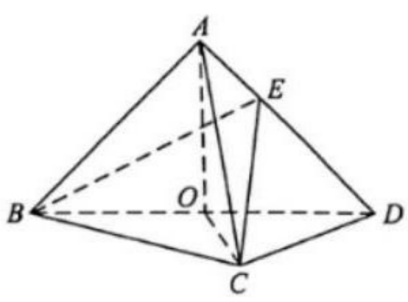
\includegraphics[width=0.35\linewidth]{a/T20}
\end{center}

	\newpage
	
	21. (12 分)
	在平面直角坐标系 $x O y$ 中,已知 点 $F_{1}(-\sqrt{17}, 0), \quad F_{2}(\sqrt{17}, 0)$, 点 $M$ 满足
	$\left|M F_{1}\right|-\left|M F_{2}\right|=2$. 记 $M$ 的轨迹为 $C$.\\
	
	(1) 求 $C$ 的方程:\\
	
	(2) 设点 $T$ 在直线 $x=\displaystyle{\frac{1}{2}}$ 上,过 $T$ 的两条直线分别交 $C$ 于 $A, B$ 两点和 $P, Q$ 两点,
	且 $|T A| \cdot|T B|=|T P| \cdot|T Q|$, 求直线 $A B$ 的斜率与直线 $P Q$ 的斜率之和.\\
	
	22.(12 分)
	已知函数 $f(x)=x(1-\ln x)$.\\
	
	(1)讨论 $f(x)$ 的单调性;\\
	
	(2)设 $a, b$ 为两个不相等的正数,且 $b \ln a-a \ln b=a-b$, 证明: $2<\displaystyle{\frac{1}{a}}+\displaystyle{\frac{1}{b}}<\mathrm{e} .$

	
\end{document}